\section{Красно-черные деревья. Балансировка (схема).}

\begin{definition}
    Красно–черное дерево --- бинарное дерево поиска, у которого каждому узлу сопоставлен дополнительный атрибут --- цвет и для которого выполняются следующие свойства:

    \begin{enumerate}
        \item Каждый узел либо красный, либо черный.
        \item Корень дерева является черным узлом.
        \item Каждый лист дерева (NULL) является черным узлом.
        \item Если узел красный, то оба его дочерних узла черные.
        \item Для каждого узла все простые пути от него до листьев, являющихся потомками данного узла, содержат одно и то же количество черных узлов.
    \end{enumerate}
\end{definition}


\begin{definition}
    Чёрной высотой $bh(x)$ вершины $x$ называется количество черных узлов на любом простом пути от узла $x$ (не считая сам узел) к листу. В соответствии со свойством 5 красно-черных деревьев черная высота узла --- точно определяемое значение, поскольку все нисходящие простые пути из узла содержат одно и то же количество черных узлов.
    Черной высотой дерева считается черную высота его корня.
\end{definition}

\begin{lemma}
Красно-черное дерево с $n$ внутренними узлами имеет высоту, не превышающую $2 \log_2(n + 1)$.
\end{lemma}

\begin{proof}
    Покажем, что поддерево любого узла $x$ содержит как минимум $2^{bh(x)} - 1$ внутренних узлов.
    Докажем это по индукции по высоте $x$.
    Если высота $x$ равна 0, то узел $x$ должен быть листом (NULL), а поддерево узла $x$ содержит не менее $2^{bh(x)} - 1 = 2^0 - 1 = 0$ внутренних узлов. 
    Теперь для выполнения шага индукции рассмотрим узел $x$, который имеет положительную высоту и представляет собой внутренний узел с двумя потомками.
    Каждый дочерний узел имеет черную высоту либо $bh(x)$, либо $bh(x) - 1$ в зависимости от того, является ли его цвет соответственно красным или черным.
    Поскольку высота потомка $x$ меньше, чем высота самого узла $x$, мы можем использовать предположение индукции и сделать вывод о том, что каждый из потомков $x$ имеет как минимум $2^{bh(x) - 1} - 1$ внутренних узлов.
    Таким образом, дерево с корнем в вершине $x$ содержит как минимум $(2^{bh(x) - 1} - 1) + (2^{bh(x) - 1} - 1) + 1 = 2^{bh(x)} - 1$ внутренних узлов, что и доказывает наше утверждение.

    Для того чтобы завершить доказательство леммы, обозначим высоту дерева через $h$. Согласно свойству 4 по крайней мере половина узлов на любом простом пути от корня к листу, не считая сам корень, должны быть черными.
    Следовательно, черная высота корня должна составлять как минимум $h/2$; значит, $$n \ge 2^{h/2} - 1$$.
    Перенося 1 в левую часть и логарифмируя, получим, что $\log_2(n + 1) \ge h/2$, или $h \le 2 \log_2(n + 1)$. 
\end{proof}

Непосредственным следствием леммы является то, что такие операции над динамическими множествами, как Search, Minimum, Maximum, Predecessor и Successor, при использовании красно-черных деревьев выполняются за время $O(\log h)$, поскольку время работы этих операций на дереве поиска высотой $h$ составляет $O(h)$, а любое красно-черное дерево с $n$ узлами является деревом поиска высотой $O(\log n)$. 

\subsection{Операции}

\subsubsection{Вставка}

По умолчанию производится вставка красной вершины. Если её предок чёрный, всё в порядке; иначе возможны следующие варианты:

\begin{center}
\begin{tabular}{|m{8cm}|m{8cm}|}
\hline
«Дядя» красный & «Дядя» черный \\ \hline
Перекрашиваем «отца» и «дядю» в чёрный цвет, а «деда» --- в красный.
Черная высота в этом поддереве одинакова для всех листьев и у всех красных вершин «отцы» черные.
Проходом вверх до корня проверяем, не нарушена ли балансировка.
Не забываем, что корень всегда черный. &
Выполняем поворот, затем перекрашивание.
Если добавляемый узел был правым потомком, то вращение --- ле-
вое, а узел становится левым потомком. \\ \hline

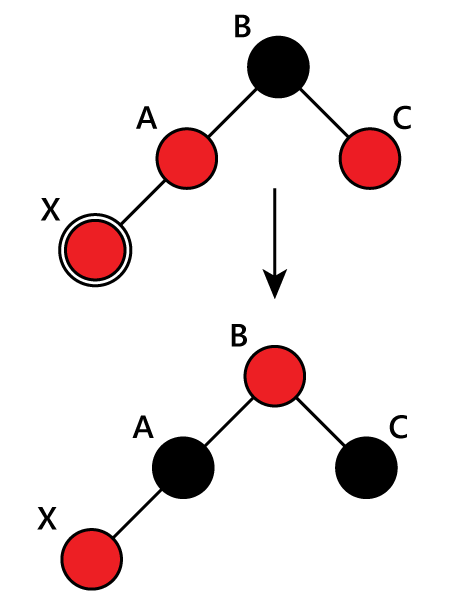
\includegraphics[width=0.4\textwidth]{img/3_1.png} 
&
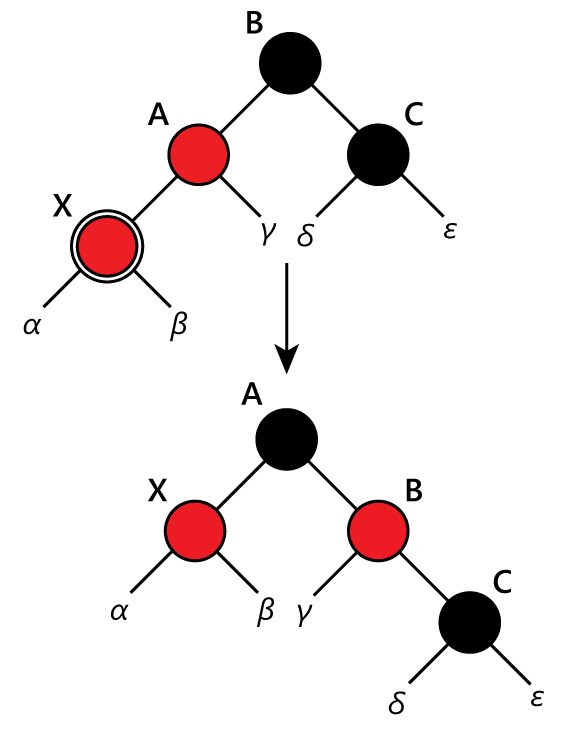
\includegraphics[width=0.4\textwidth]{img/3_2.png} \\ \hline

\end{tabular}
\end{center}

\subsubsection{Удаление}

При удалении вершины могут возникнуть три случая в зависимости от количества её детей:
\begin{enumerate}
    \item Если у вершины нет детей, то изменяем указатель на неё у родителя на NULL.
    \item Если у неё только один ребёнок, то делаем у родителя ссылку на него вместо этой вершины.
    \item Если же имеются оба ребёнка, то находим вершину со следующим значением ключа.
    У такой вершины нет левого ребёнка (так как такая вершина находится в правом поддереве исходной вершины и она самая левая в нем, иначе бы мы взяли ее левого ребенка.
    Иными словами, сначала мы переходим в правое поддерево, а после спускаемся вниз в левое до тех пор, пока у вершины есть левый ребенок).
    Удаляем уже эту вершину описанным во втором пункте способом, скопировав её ключ в изначальную вершину.
\end{enumerate}

Так как при удалении красной вершины свойства дерева не нарушаются, то восстановление балансировки потребуется только при удалении чёрной.
Рассмотрим ребёнка удалённой вершины.

\begin{center}
\begin{tabular}{|m{10cm}|m{7cm}|}
\hline
Если брат этого ребёнка красный, то делаем вращение вокруг ребра между отцом и братом, тогда брат становится родителем отца. Красим его в чёрный, а отца — в красный цвет, сохраняя таким образом черную высоту дерева.
Хотя все пути по-прежнему содержат одинаковое количество чёрных узлов, сейчас $x$ имеет чёрного брата и красного отца.
Таким образом, мы можем перейти к одному из следующих случаев.
& 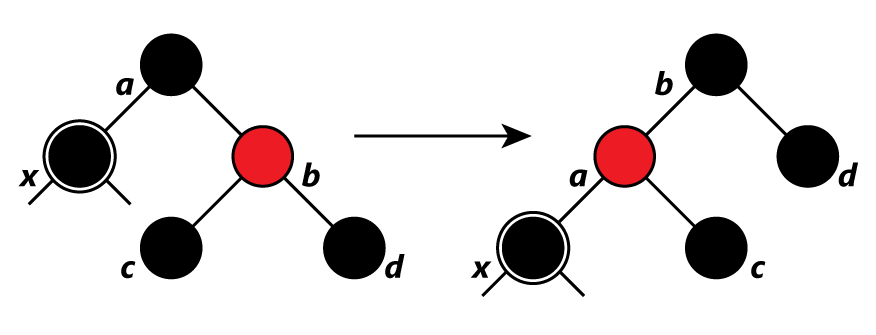
\includegraphics[width=0.4\textwidth]{img/3_3.png} \\ \hline
Оба ребёнка у брата чёрные.
Красим брата в красный цвет и рассматриваем далее отца вершины.
Делаем его черным, это не повлияет на количество чёрных узлов на путях, проходящих через $b$, но добавит один к числу чёрных узлов на путях, проходящих через $x$, восстанавливая тем самым влиянние удаленного чёрного узла.
Таким образом, после удаления вершины черная глубина от отца этой вершины до всех листьев в этом поддереве будет одинаковой. 
& 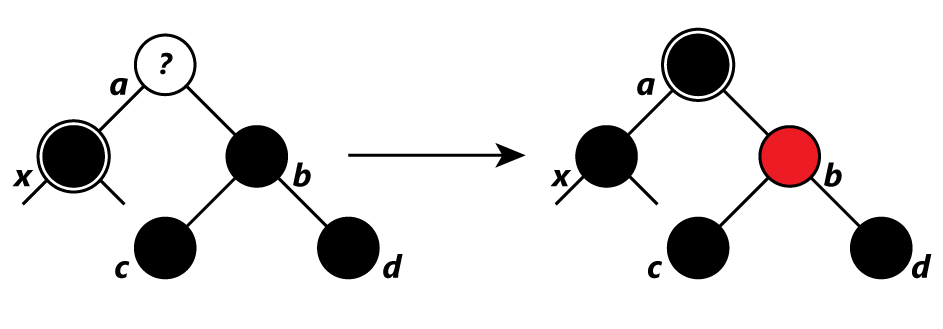
\includegraphics[width=0.4\textwidth]{img/3_4.png} \\ \hline
Если у брата правый ребёнок чёрный, а левый красный, то перекрашиваем брата и его левого сына и делаем вращение.
Все пути по-прежнему содержат одинаковое количество чёрных узлов, но теперь у $x$ есть чёрный брат с красным правым потомком, и мы переходим к следующему случаю.
Ни $x$, ни его отец не влияют на эту трансформацию.
& 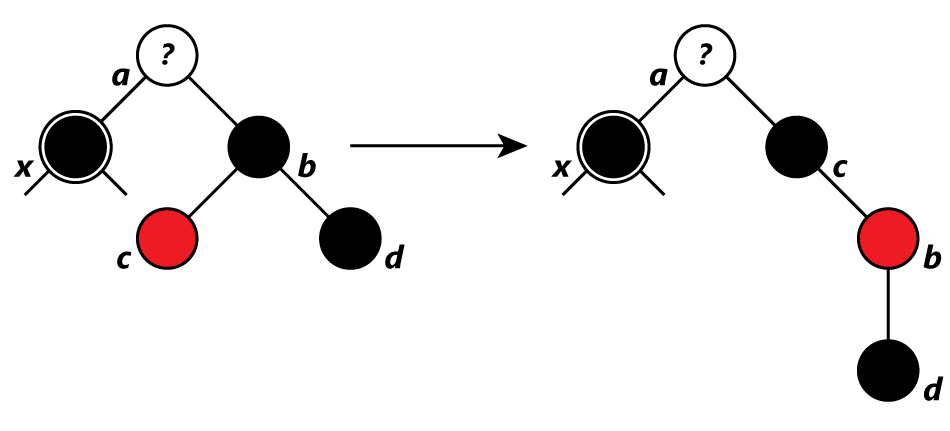
\includegraphics[width=0.4\textwidth]{img/3_5.png} \\ \hline
Если у брата правый ребёнок красный, то перекрашиваем брата в цвет отца, его ребёнка и отца — в чёрный, делаем вращение.
Поддерево по-прежнему имеет тот же цвет корня, поэтому свойства 3 и 4 не нарушаются.
Но у $x$ теперь появился дополнительный чёрный предок: либо $a$ стал чёрным, или он и был чёрным и $b$ был добавлен в качестве чёрного дедушки.
Таким образом, проходящие через $x$ пути проходят через один дополнительный чёрный узел.
Выходим из алгоритма. 
& 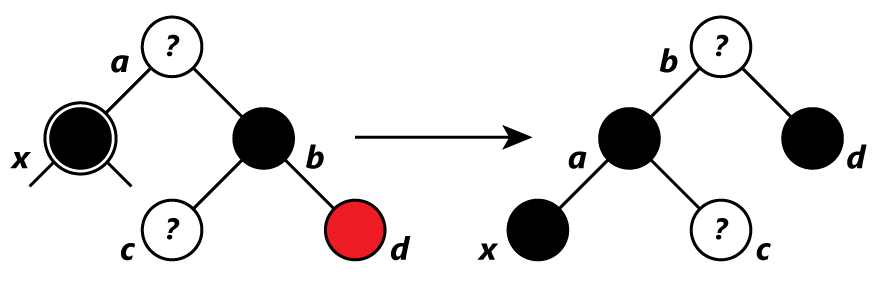
\includegraphics[width=0.4\textwidth]{img/3_6.png} \\ \hline

\end{tabular}
\end{center}

Продолжаем тот же алгоритм, пока текущая вершина чёрная и мы не дошли до корня дерева.
